\documentclass[
  bibliography=totoc,     % Literatur im Inhaltsverzeichnis
  captions=tableheading,  % Tabellenüberschriften
  titlepage=firstiscover, % Titelseite ist Deckblatt
]{scrartcl}

\usepackage{fixltx2e}
\usepackage[aux]{rerunfilecheck}

\usepackage{polyglossia}
\setmainlanguage{german}

\usepackage{amsmath}
\usepackage{amssymb}
\usepackage{mathtools}

\usepackage{fontspec}
\defaultfontfeatures{Ligatures=TeX}

\usepackage[
  math-style=ISO,
  bold-style=ISO,
  sans-style=italic,
  nabla=upright,
  partial=upright,
]{unicode-math}

\usepackage[autostyle]{csquotes}

\usepackage[
  locale=DE,                   % deutsche Einstellungen
  separate-uncertainty=true,   % Immer Fehler mit \pm
  per-mode=symbol-or-fraction, % m/s im Text, sonst Brüche
]{siunitx}

\usepackage[version=3]{mhchem}

\usepackage{xfrac}

\usepackage[section, below]{placeins}
\usepackage[
  labelfont=bf,        % Tabelle x: Abbildung y: ist jetzt fett
  font=small,          % Schrift etwas kleiner als Dokument
  width=0.9\textwidth, % maximale Breite einer Caption schmaler
]{caption}
\usepackage{subcaption}
\usepackage{graphicx}
\usepackage{grffile}

\usepackage{float}
\floatplacement{figure}{htbp}
\floatplacement{table}{htbp}

\usepackage{booktabs}

\usepackage[
  unicode,
  pdfusetitle,    % Titel, Autoren und Datum als PDF-Attribute
  pdfcreator={},  % PDF-Attribute säubern
  pdfproducer={}, % "
]{hyperref}
\usepackage{bookmark}
\usepackage[shortcuts]{extdash}


\title{Entwicklung eines mobil lauffähigen microblog-Systems mit flask und
CouchDB}
\subtitle{Ein Projekt der PeP et Al. Sommerakademie 2014}
\date{24. -- 31. August 2014}

\author{
    Kevin Heinicke
}

\begin{document}

\maketitle
\tableofcontents

\section{Einleitung}
Aus einer ersten Idee, ein mobiles, drahtloses Netzwerk auf einem
\textsc{RaspberryPi} (RasPi) einzurichten, um damit selbst auf den höchsten
österreicher Bergen eine gewisse digitale Grundversorgung bereitzustellen
ist schnell das Projekt eines minimalistischen Blogs entstanden.
Hiermit sollte eine etwas andere Perspektive einer SoAk-Dokumentation
entstehen, in der jeder Teilnehmer jederzeit seine Eindrücke in der Gruppe
veröffentlichen kann.

\section{Technische Umsetzung}
Um die Idee zu realisieren wird ein RasPi verwendet,
der mit Hilfe eines USB-Akkus und eines WLAN-Sticks als mobiler
Accesspoint dient.
Eine erste Abschätzung für die Laufzeit des Systems bei Akkubetrieb lässt
eine dauerhafte Nutzung für etwa 7 Stunden erwarten.
\begin{figure}[h]
  \centering
  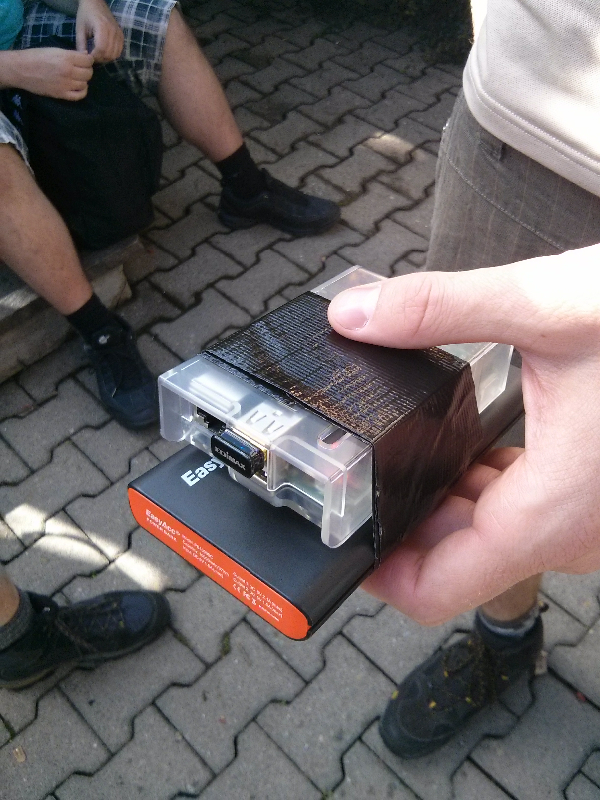
\includegraphics[width=0.4\linewidth]{images/raspi1.jpg}
  \caption{Mobiler Aufbau des RasPis mit angeschlossenem Akku
  und WLAN-Dongle.}
  \label{fig:raspi}
\end{figure}

Das Blogsystem beruht auf dem \textsc{python}-Framework \textsc{flask},
welches die schnelle Erstellung einer Website mit allen wichtigen Funktionen
ermöglicht.
Die flask-app wird maßgeblich zur Kommunikation mit der objektorientierten
\textsc{CouchDB}-Datenbank genutzt.  Der Quellcode des Systems ist auf
\href{https://github.com/bixel/microblog}{github.com/bixel/microblog}
zugänglich.
Die Nutzung einer objektorientierten Datenbank ermöglicht eine besonders
freie Entwicklung, was für den nachträglichen Einbau von Zusatzfunktionen
ausgesprochen hilfreich ist.

Das erste Ziel der Software ist die Speicherung von Text- und Bildbeiträgen
von verschiedenen Nutzern, sowie die chronologische Wiedergabe dieser Beiträge.
Für die Erstellung einer ansprechenden, interaktiven Oberfläche
stellt sich das CSS- und JavaScript-Framework \textsc{bootstrap} mit der 
JavaScript-Bibliothek \textsc{jQuery} als sehr hilfreich
heraus.

\section{Ergebnisse}
Insgesamt war die Einrichtung des microblogs ein voller Erfolg.
Über die Dauer der Reise wurden insgesamt 208 Beiträge verfasst.
Der beliebteste Beitrag war mit insgesamt \num{8} Likes ein Bild
des Teams Astrofotografie.
Besonders beliebt waren ebenfalls Aufnahmen aus dem Bereich
\enquote{Speisen und Getränke}.
Während der großen Wanderung zur Mittagsspitze wurden insgesamt \num{32}
Bilder hochgeladen und der Akku des Systems verlor in dieser Zeit
lediglich etwa \SI{50}{\percent} der Ladung.

\section{Probleme und Verbesserungsmöglichkeiten}
Nach der Umsetzung der ersten Mindestanforderungen in einer
Entwicklungsumgebung stellt sich die Installation auf dem RasPi als
langwierige Problemsuche dar.
Es musste zunächst einige Erfahrung in der Einrichtung der genutzten
Software auf einem Minicomputer, wie dem RasPi gesammelt werden,
bevor das System zuverlässig arbeitete.

Noch während der Anreise wurden dem System weitere Features, wie eine
\enquote{Likefunktion} und die Möglichkeit, Beiträge zu verstecken
eingearbeitet.
Insgesamt stellte sich jedoch die Pflege des Systems bei laufendem Betrieb als
zu zeitintensiv für eine solche Reise heraus, weshalb die Umsetzung der
unzähligen -- gute und spaßige -- Anregungen für neue Funktionen
auf einen späteren Zeitpunkt verschoben werden mussten.

Nach Ankunft zeigte sich zudem, dass die Leistung des RasPi nach einiger
Nutzung des Systems an dessen Grenzen stoß. Besonders die WLAN-Funktionalität
war für die Räumlichkeiten nicht ausreichend und musste durch externe Router
verstärkt werden, was weitere Schwierigkeiten mit dem benutzten DNS-Server
mit sich brachte und insgesamt die Benutzbarkeit des microblogs reduziert hat.

\end{document}
